\chapter{Context-aware and recommender systems}
\label{cha:recommenders}

Both topics---context-aware systems and recommender systems---have been growing more and more popular among researchers lately. Both can be discerned to have approximately equivalent curves on accumulated paper and citation counts in time, as shown in \cref{fig:scholar-context-aware} and \cref{fig:scholar-recommender-systems}. Result were obtained after processing 8098 and 3420 papers, respectively, that is all papers that have been found for ``recommender systems'' and ``context-aware'' queries in Google Scholar and Microsoft Academic Search. The S-like shape of the curves might suggest that the topic has already been researched thoroughly.

\begin{figure}
	\centering
	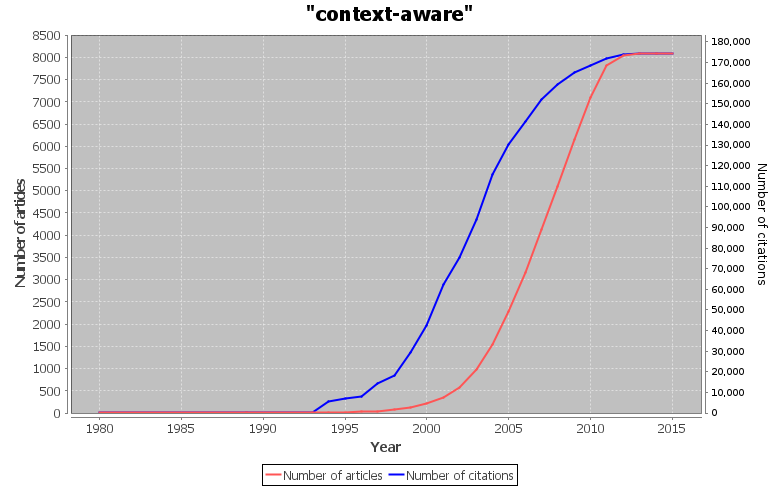
\includegraphics[width=\textwidth]{scholar-context-aware}
	\caption{Google Scholar and Microsoft Academic Search accumulated trending for ``context-aware'' query \cite{Rus:scholar-trends}.}
	\label{fig:scholar-context-aware}
\end{figure}

\begin{figure}
	\centering
	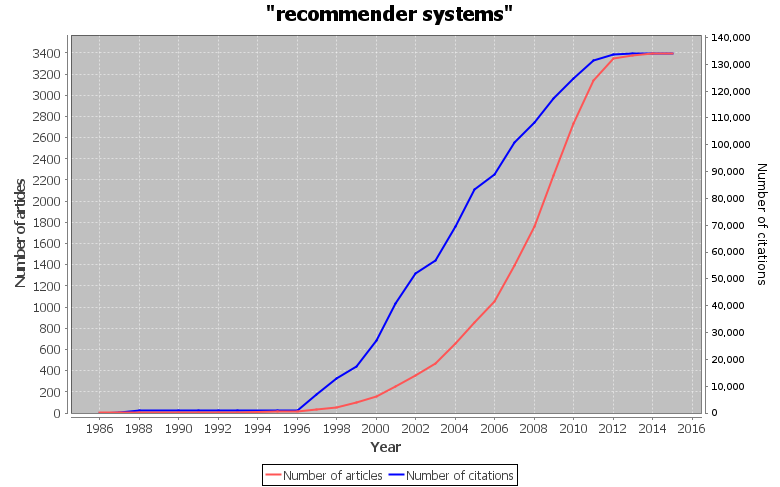
\includegraphics[width=\textwidth]{scholar-recommender-systems}
	\caption{Google Scholar and Microsoft Academic Search accumulated trending for ``recommender systems'' query \cite{Rus:scholar-trends}.}
	\label{fig:scholar-recommender-systems}
\end{figure}

\section{Context-aware systems}

d